\section{Introduction}~\label{sec:introduction}

\todo{Spiel about reversible computing and logical reversibility}
\todo{Spiel about using groupoids for denotational semantics}

\subsection*{Quantum Circuits}

Most current quantum algorithms start with generating superpositions, doing a unitary transformation, and then doing a measurement. The middle stage is essentially a reversible classical computation (performed in a quantum-parallel fashion). For example, in the case of Shor's algorithm, this middle block consists of implementing a reversible version of modular exponentiation $f(x) = a^x `mod` N$ for some fixed $a$ and $N$. As explained in standard accounts of the algorithm (e.g., the Qiskit implementation), such efficient modular exponentiation circuits are not straightforward and are the bottleneck in Shor’s algorithm. Typical derivations of the circuit start from elementary gates, build a circuit for modular addition, which is used to build a circuit for modular multiplication, and then finally a circuit for modular exponentiation taking care at each step to avoid the exponential blowup~\cite{shorefficient}. Ultimately however the circuit has a simple specification as a \emph{permutation}. For example, consider the function $f(r) = 11^{r} \mod 15$. Using the Toffoli construction~\cite{Toffoli:1980}, we can embed this function $f$ into a reversible function $g$, shown below, such that $g(r,0) = (r,f(r))$:

\[\begin{array}{rcll}
    g(r,h) & = & (r,h+1)  & \mbox{when~$r$~even~and~$h$~even}                          \\
    (r,h)  & = & (r,h-1)  & \mbox{when~$r$~even~and~$h$~odd}                           \\
    g(r,h) & = & (r,11-h) & \mbox{when~$r$~odd~and~$4 > h \geq 0$~or~$12 > h \geq 8$}  \\
    g(r,h) & = & (r,19-h) & \mbox{when~$r$~odd~and~$8 > h \geq 4$~or~$16 > h \geq 12$}
  \end{array}\]

Wouldn't it be simpler to write this permutation and automatically derive a circuit from it? This is exactly what we accomplish. We can take the permutation above, generate a circuit from it, \emph{and most importantly} generate a proof of correctness along with the circuit. As part of the infrastructure we provide a sound and complete calculus of reversible functions that can be used to (i) generate circuits from permutations like above, (ii) translate circuits to a normal form, (iii) reason about equivalence of circuits, (iv) and provide a framework for reasoning about trade-offs among optimizing tranformations.

Technically, the main result is a soundness and completeness theorem relating a 2-level reversible programming language with a univalent universe of finite types expressed as a weak groupoid in the metalanguage of HoTT. On the HoTT we start with a univalent subuniverse specification of finite types, equivalences between them, and homotopies between the equivalences. This is a concise description of everything we need to know about circuits and transformations among them. Along the way, we \ldots \note{copy relevant pieces from below}


\subsection*{Outline and Contributions}

\begin{itemize}[leftmargin=*]
  \item We take the $\PiLang$ family of reversible languages~\cite{jamesInformationEffects2012} and show how to encode
        various boolean reversible circuits in the language. The circuits are implemented using 1-combinators in the
        language, and circuit optimisations are realised as 2-combinators between these reversible programs.
  \item We show how to encode reversible circuits on a fixed number of bits as permutations of finite sets with the
        appropriate cardinality. We observe that reversible programs can be translated to bijective functions between
        finite sets and equality of reversible programs can be witnessed as extensional equality of these bijective
        functions.
  \item We review a few basics of Homotopy Type Theory~\cite{univalentfoundationsprogramHomotopyTypeTheory2013}, and
        exhibit some results that we use in our technical development. We define the notion of a universe \`{a} la
        Tarski internally in HoTT, which is given by a type for codes $U$ and a decoding function to a univalent
        universe $\El : U \to \UU$. We say that this universe is univalent, if the decoding fibration is univalent, that
        is, the decoding function $\El$ reflects the path space of the underlying univalent universe. We exhibit some
        examples of univalent subuniverses, in particular, we define the subuniverse of finite types, $\UFin$, which
        classifies all finite types, and show that it is univalent. Using this, we establish a characterisation of the
        path space of the universe of finite types.
  \item We observe that 1-paths in $\UFin$ are permutations on finite sets with a fixed cardinality $n$, given by
        $\Aut[\Fin[n]]$, which produces the permutation group on $\Fin[n]$, or the symmetric group $\Sn$. We then
        proceed to give a presentation of $\Sn$ using generators and relations, by defining the Coxeter relations. We
        build a rewriting system using the Coxeter relations on the set of words $\List[\Fin[n]]$, and show that it is
        (locally) confluent and strongly normalising. We define the the symmetric group $\Sn$ to be the set-quotient of
        $\List[\Fin[n]]$ by the Coxeter relations, and show that it produces a group presentation, as a quotient of the
        free group. Using our strongly normalising rewriting system, we establish that normal forms for words in $\Sn$
        are Lehmer codes~\cite{lehmerTeachingCombinatorialTricks1960}, which are a convenient and compact representation
        of permutations for permutations. Finally, we show that there is an equivalence between Lehmer codes and
        permutations $\Aut[\Fin[n]]$ given by the Lehmer encode-decode algorithm.
  \item Finally, we show how to interpret the language $\PiLang$ into our groupoid $\UFin$, in stages. First we define a
        subset of the language $\PiPlusLang$ which only includes the additive monoidal structure. We translate $\PiLang$
        programs to $\PiPlusLang$ by defining multiplication as repeated addition. Then, we further define a normalised
        form for for this language called $\PiHatLang$, which has normalised 1-combinators and 2-combinators
        corresponding to adjacent transpositions. We show that $\PiPlusLang$ can be translated to $\PiHatLang$ and back,
        using adjacent transpositions to generate arbitrary swaps. Then, we show how to interpret this language
        $\PiHatLang$ into $\UFin$ -- the 1-combinators are translated into permutations via words in $\Sn$, and
        2-combinators are interpreted as 2-paths in $\UFin$. We further show how to quote back a permutation in $\UFin$
        into a 1-combinator using the normal form for words in $\Sn$.
  \item We give some applications of this translation by showing how to normalise a circuit written in $\PiLang$ to a
        normal form in $\PiPlusLang$ and $\PiHatLang$, which uses fewer gates.~\todo{Here, or earlier?}
\end{itemize}

Our results are formalised in the proof assistant Agda using the HoTT-Agda library.

\note{Novel interpretation of the univalence axiom, operational and denotational semantics and adequacy.}

\todo{Redo this figure}
\begin{center}
  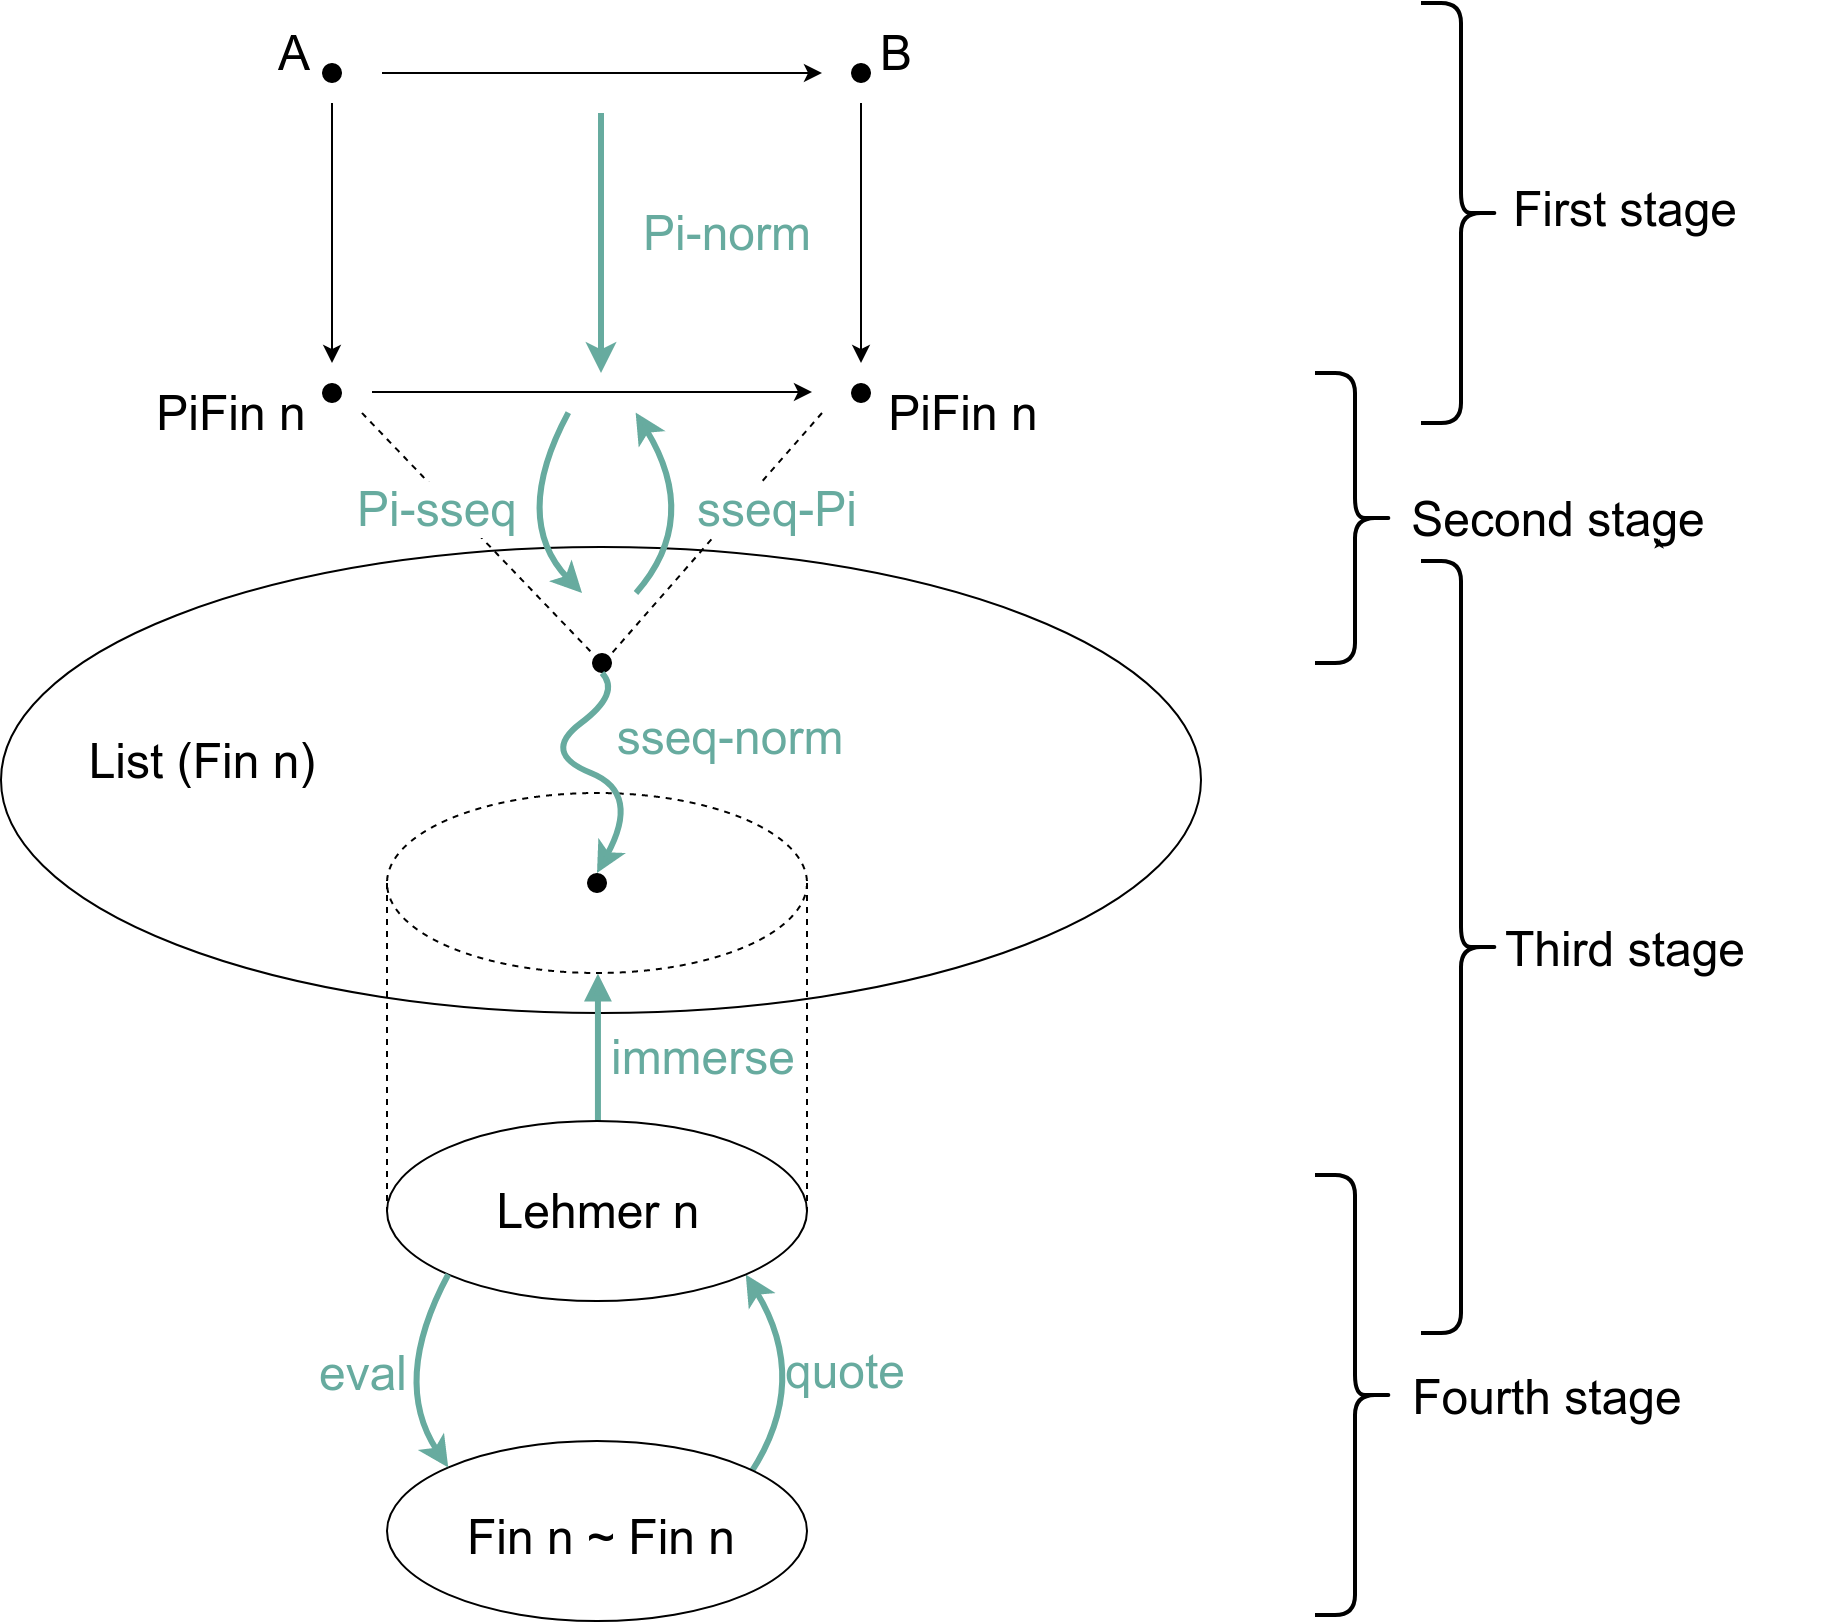
\includegraphics[scale=0.3]{outline.png}
\end{center}


%%% Local Variables:
%%% mode: latex
%%% TeX-master: "main"
%%% fill-column: 120
%%% End:
